\documentclass{article}
\usepackage[utf8]{inputenc}
\usepackage[left=1cm,right=0.5cm,bottom=0.5cm,top=0.5cm]{geometry}
\usepackage{setspace}
\usepackage{graphicx}
\setstretch{0}

\begin{document}
\section{Wave Basics}
\vspace{-2mm}
Fixed end = inverted amplitude for reflected wave, free end = not inverted \\
\textbf{Waves} | $y(x, t) = A\cos{(kx - \omega t)}$,
    $k = \frac{2\pi}{\lambda}$,
    $\omega = 2\pi f$,
    $v = \lambda f$ \\
\textbf{Power} | 
$P(x, t) = -F \frac{\partial y}{\partial x} \cdot \frac{\partial y}{\partial t} = FA^2kw\sin^2{(kx - \omega t)}$,
    $P_{avg} = \frac{FA^2k \omega}{2}$ \\
\textbf{Wave Intensity} | $\frac{I_1}{I_2} = \frac{r_2^2}{r_1^2}$ where I = intensity, r = distance (radius) from source \\
\textbf{Normal modes} | $f_n = \frac{nv}{2L} = nf_1$

\vspace{-5mm}
\section{Sound (Longitudinal waves)}
\vspace{-4mm}
The first overtone is the second harmonic, the first harmonic is the fundamental frequency. \\
The speed of sound is around 344 $\frac{m}{s}$. \\
\textbf{Pressure} | $p(x, t) = BkA\sin{(kx - \omega t)}$ where B = bulk modulus, $p_{max} = BkA$ \\
\textbf{Speed of sound} 
\begin{enumerate}
    \vspace{-4mm}
    \item Liquid: $v = \sqrt{\frac{B}{\rho}}$ where B = bulk mod, $\rho$ = density
    \vspace{-3mm}
    \item Solid: $v = \sqrt{\frac{Y}{\rho}}$ where Y = young's modulus
    \vspace{-3mm}
    \item Gas: $v = \sqrt{\frac{\gamma RT}{M}}$ where $\gamma$ = heat capacity ratio, R = 8.31, T = temp in K, M = molar mass
\end{enumerate}
\vspace{-3mm}
\textbf{Intensity} | $I = \frac{1}{2}B \omega KA^2$ = $\frac{p_{max}}{2 \rho v}$, 
    \textbf{Decibels}: $\beta = (10dB) \log{(\frac{I}{10^{-12}})}$ \\
\textbf{Standing waves} | 2 open ended pipe: $f_n = \frac{nv}{2L}$, 
    1 open (stopped) pipe: $f_n = \frac{nv}{4L}$ \\
\textbf{Beats} | $f_{beat} = f_a - f_b$ where $f_a > f_b$ \\
\textbf{Doppler} | $f_L = \frac{v + v_L}{v + v_s} f_s$, $+v_L$ if $v$ is STRICTLY  same direction as listener toward src, else $-$; same w/ $v_s$ \\
\vspace{-5mm}
\section{Light}
\vspace{-2mm}
Speed of light is $c = 2.99 \cdot 10^8 \frac{m}{s}$. Idx of refract. of water = 1.333, ethanol = 1.36, air = 1 \\
\textbf{Idx of refraction} | $n = \frac{c}{v}$ where n is the index, v is the speed inside the material. \\
\textbf{Law of reflection} | $\theta_r = \theta_a$ where both are measured from the normal of the surface. \\
\textbf{Law of refraction} | $n_a\sin{(\theta_a)} = n_b\sin{(\theta_b)}$, calc. wavelen change: $\lambda = \frac{lambda_0}{n}$ where $\lambda_0$ = vacuum wavelen, n = idx of refract. \\
\textbf{Total internal reflection} | where no refraction occurs: $\sin{(\theta_{crit})} = \frac{n_b}{n_a}$, $\theta_{crit}$ being min. angle for no refract. \\
\textbf{Polarization} | $I = I_{max}\cos^2{(\phi)}$ where $I_{max}$ = max intensity, $\phi$ = angle between polarization axis \& polarizing axis of analyzer
\textbf{Polarization by reflect} | $\tan{(\theta_p)} = \frac{n_b}{n_a}$ where $\theta_p$ = angle where reflected light is 100\% polarized \\
\vspace{-5mm}
\section{Geometric Optics}
\vspace{-2mm}
\textbf{General rules} | ALWAYS $s > 0$. $m < 0 \rightarrow s' > 0$. The sign for $s'$ is positive if on the same side as outgoing rays, else negative.\\
\textbf{Real image} | rays of interest pass through the image point, \textbf{Virtual image} | rays of interest never pass through image point \\
\textbf{Magnification} | $m = \frac{y'}{y} = -\frac{s'}{s}$ where prime = img, y = obj height, s = obj. distance \\
\textbf{Object-image relation} | $\frac{1}{s} + \frac{1}{s'} = \frac{1}{f} = \frac{2}{R}$ where f = focal pt, R = radius of curvature (mirror)\\
\textbf{Tips for drawing ray diagrams} | Draw up to 4 rays with the following properties:
\begin{enumerate}
    \vspace{-2mm}
    \item Ray from obj. height parallel to optic axis (passes thru focal pt.)
    \vspace{-3mm}
    \item Ray from obj. height reflecting at optic axis
    \vspace{-3mm}
    \item Ray between obj. height and focal pt.
    \vspace{-3mm}
    \item (OPTIONAL) Ray thru c (center of curvature, reflects back on the same axi)
\end{enumerate}
\vspace{-3mm}
\textbf{Concave mirror rules}
\begin{enumerate}
    \vspace{-2mm}
    \item Focal pt. is positive (in front of mirror)
    \vspace{-3mm}
    \item Rays parallel to optic axis hitting mirror will always pass thru focal pt.
    \vspace{-3mm}
    \item Rays hitting the optic axis will reflect w/ the same angle it came in from.
    \vspace{-3mm}
    \item Rays passing thru the focal pt. will reflect parallel to optic axis.
    \vspace{-3mm}
    \item If object dist. is shorter than focal pt., image will be virtual erect.
    \vspace{-3mm}
    \item If object dist. is further than focal pt., image will be real inverted.
\end{enumerate}
\vspace{-3mm}
\textbf{Convex mirror rules}
\begin{enumerate}
    \vspace{-2mm}
    \item Focal pt. is negative (behind the mirror itself)
    \vspace{-3mm}
    \item Rays aimed at the focal pt. will reflect parallel to optic axis.
    \vspace{-3mm}
    \item Rays parallel to optic axis will reflect aimed directly opposite of the focal pt.
    \vspace{-3mm}
    \item Rays hitting the optic axis will reflect w/ same angle as incoming.
\end{enumerate}
\vspace{-2mm}
\textbf{Lenses}
\begin{enumerate}
    \vspace{-2mm}
    \item You can use the same rules but visualize refraction instead.
    \vspace{-3mm}
    \item Converging lens = convex, diverging lens = concave.
    \vspace{-3mm}
    \item Convex | refracting rays hit a focal pt, focal pt. is always positive
    \vspace{-3mm}
    \item Concave | refracting rays parallel to axis, focal pt. always negative
    \vspace{-3mm}
    \item When drawing ray diagrams, 2 rays shouldn't pass through the same focal. (there is 1 focal per side).
\end{enumerate}
\pagebreak
\textbf{Mirror visuals} \\
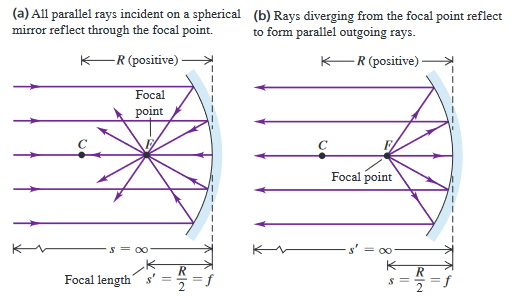
\includegraphics[width=7cm]{concave.png}
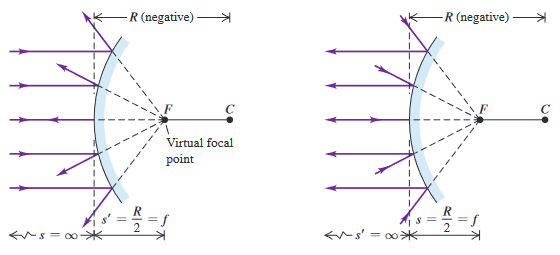
\includegraphics[width=7cm]{convex.png}
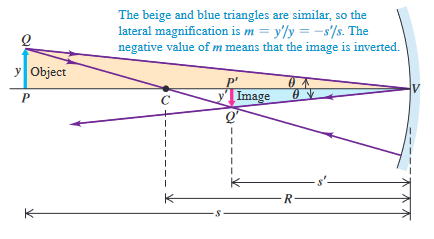
\includegraphics[width=6cm]{mirror.png} \\
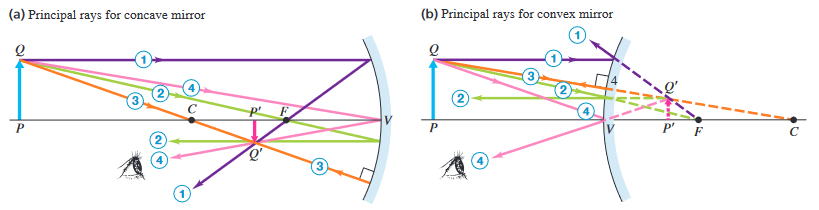
\includegraphics[width=20cm]{principal.png} \\
\textbf{Lens visuals} \\
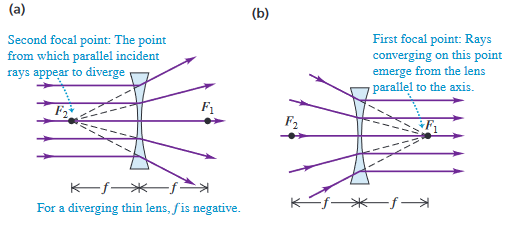
\includegraphics[width=10cm]{concave_lens.png} 
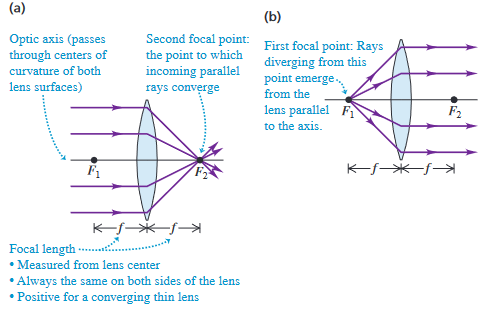
\includegraphics[width=10cm]{convex_lens.png} \\
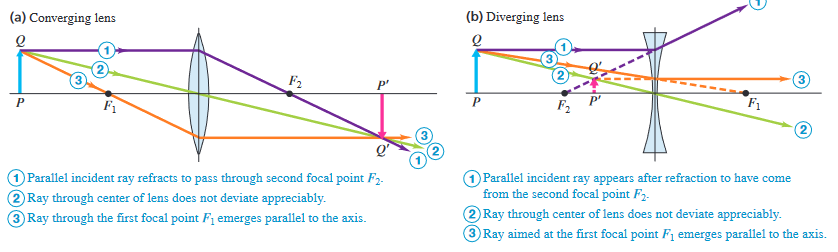
\includegraphics[width=20cm]{principal_lens.png} \\
\end{document}
